\documentclass[12pt,
    a4paper,
    headinclude,
    footinclude]{scrreprt}

    %plainfootsepline

\usepackage{blindtext}
\usepackage[utf8]{inputenc}
\usepackage{setspace}
\usepackage[ngerman]{babel}
\usepackage[ngerman, num]{isodate}
\usepackage[left=3cm,right=2cm,top=2.8cm,bottom=2.4cm]{geometry}

\usepackage[style=numeric]{biblatex}
\usepackage[babel,german=guillemets]{csquotes}

\usepackage{float}

\usepackage{graphicx}
\usepackage{tabularx}
\usepackage{caption}

\usepackage{listings}
\usepackage{color}
\renewcommand{\lstlistingname}{Auflistung}
\renewcommand{\lstlistlistingname}{Auflistungsverzeichnis}
\definecolor{hellgrau}{rgb}{.95,.95,.95}
\definecolor{grau}{rgb}{.9,.9,.9}
\lstset{
	%backgroundcolor=\color{hellgrau},
	%backgroundcolor=\color{blue}
	%basicstyle=\scriptsize\ttfamily,
	%keywordstyle=\bfseries\ttfamily\color{orange},
	%stringstyle=\color{green}\ttfamily,
	%commentstyle=\color{middlegray}\ttfamily,
	%emph={square}, 
	%emphstyle=\color{blue}\texttt,
	%emph={[2]root,base},
	%emphstyle={[2]\color{yac}\texttt},
	showstringspaces=false,
	%flexiblecolumns=false,
	tabsize=1,
	numbers=left,
	%numberstyle=\tiny,
	numberblanklines=false,
	stepnumber=1,
	%numbersep=0pt,
	xleftmargin=20pt,
	frame=l,
	framesep=4.5mm,
	framexleftmargin=2.5mm,
	fillcolor=\color{grau},
	rulecolor=\color{grau},
	%numberstyle=\normalfont\tiny\color{numbercolor}
}

\usepackage{wrapfig}

\bibliography{res33.bib} 


\AtBeginDocument{\setlength{\glslistdottedwidth}{.15\columnwidth}}
\usepackage[acronyms,style=listdotted,shortcuts,translate=babel,toc]{glossaries}
%\GlsSetXdyLanguage{german}                         % Deutsche Spracheinstellung (nicht ngerman!) 
%\GlsSetXdyCodePage{duden-utf8}                     % Deutsche Codierung 
%\newglossarystyle{glosstil}{                     % neuer Stil mit Namen
%	\glossarystyle{listdotted}                           % basierent auf Stil long
%	\renewenvironment{theglossary}
%	{\begin{longtable}
%			{@{}p{0.1\textwidth} p{0.8\textwidth}}}   % einstellen der Spaltenbreiten
%		{\end{longtable}}
%	\renewcommand*{\glsgroupskip}{}               % keine Gruppenumbrüche
%} 

%\renewcommand*{\glsgroupskip}{}
%\makeglossaries
% \newacronym{TCP}{TCP}{Transmission Control Protocol}
% \newacronym{FTP}{FTP}{File Transfer Protocol}
% \newacronym{IP}{IP}{Internet Protocol}
% \newacronym{DNS}{DNS}{Domain Name Server}
% \newacronym{WWW}{WWW}{World Wide Web}
% \newacronym{HTTP}{HTTP}{Hypertex Transfer Protocol}
% \newacronym{HTTPS}{HTTPS}{Hypertex Transfer Protocol Secure}
% \newacronym{HTML}{HTML}{Hypertex Markup Language}
% \newacronym{XML}{XML}{Extensible Markup Language}
% \newacronym{WS}{WS}{WebSocket}
% \newacronym{ASCII}{ASCII}{American Standard Code for Information Interchange}
% \newacronym{UTF-8}{UTF-8}{8-Bit Universal Character Set Transformation Format}
%\usepackage{etoolbox}

%\newacronym{}{}{}

%\usepackage{fontspec}
%\setmainfont{Times New Roman}
%\usepackage[T1]{fontenc}
%\newcommand{\changefont}[3]{
%\fontfamily{#1} \fontseries{#2} \fontshape{#3} \selectfont}

%\renewcommand{\chapterpagestyle}{scrheadings}


%kopf und fusszeile
%\usepackage[headsepline]{scrpage2}
%\pagestyle{scrheadings} 
%\setlength{\footskip}{8mm}
%\clearscrheadings
%\ihead{\leftmark}
%\ohead{\rightmark}
%\automark[section]{chapter}
%\cfoot{\pagemark}
%kopf und fusszeile

%Schriftart sfffamily serifenlos
\setkomafont{pageheadfoot}{\normalfont\rmfamily\bfseries}

\setkomafont{chapterentry}{\normalfont\rmfamily\bfseries}
%\setkomafont{sectionentry}{\normalfont\rmfamily}

\setkomafont{chapter}{\huge\normalfont\rmfamily\bfseries}
\setkomafont{section}{\Large\normalfont\rmfamily\bfseries}
%Schriftart



\DefineBibliographyStrings{ngerman}{%
	bibliography={Literaturverzeichnis}% NICHT references
}


\author{Martin Braun}
\title{Redfish}

\begin{document}
	\onehalfspacing
	\monthyearsepgerman{\,}{\,}
	\setcounter{tocdepth}{2}
	

	
	\begin{titlepage}
	
		\begin{center}
			~\\[2cm]
			Berufsakademie Sachsen \\
			Staatliche Studienakadamie Leipzig \\
			Studiengang Informatik \\
           	Evolutionäre Algorithmen\\ [2.4cm]
           
			\begin{Large}
			    \textbf{Binäre und reelle Kodierung im Vergleich bei der näherungsweisen Berechnung des globalen Minimums der Griewank-Funktion} \\[2.4cm]
			\end{Large}
			
			\doublespacing


		\end{center}
		\onehalfspacing
		\begin{tabbing}
			Eingereicht von: \= ~ \= ~ \= ~ \= Georg Andrassy \hspace*{3cm} Matrikelno: 5000593  \\
			\> \> \> \> Martin Braun \hspace*{3.4cm} Matrikelno: 5000562 \\
			\\

		\end{tabbing}
		\vspace*{\fill}
		Leipzig, \today
		
	\end{titlepage}
    
    %Inhaltsverzeichnis
%    \pagenumbering{Roman}
%    \tableofcontents 	
    \clearpage
    %Inhaltsverzeichnis
        
    \pagenumbering{arabic}
    \setcounter{page}{2}
    
\section*{1. Einführung}	\onehalfspacing

Zur näherungsweisen Berechnung des globalen Minimums der Griewank-Funktion: \[f(x) = 1 +  \sum_{i=1}^n \frac{x_i^{2}}{400n} -  \prod \limits_{i=1}^n cos \left(\frac{x_i}{\sqrt{i}}\right)\] wird ein evolutionärer Algorithmus eingesetzt. Dieser Algorithmus wird vor allem im Hinblick auf den Einfluss  unterschiedlicher Kodierungsarten sowie stabiler und wachsender Populationsgrößen auf den Fitnesswert der Individuen untersucht. Zusätzlich wird die Differenz zwischen dem besten und dem schlechtesten Individuum in der Population als Maß der Streuung betrachtet. Die Minimierung der Griewank-Funktion wird für drei verschiedene n (n=5, 20, 50) im Wertebereich von -512 bis 511 getestet:




\section*{2. Umsetzung}


Für die Umsetzung wird folgender Algorithmus verwendet:

\begin{enumerate}
	\item Erzeugung der Startpopulation 
	\begin{itemize}
		\item fixe Ausgangspopulation mit X Anfangsindividuen
	\end{itemize}
	\item Elternselektion
		\begin{itemize}
		\item Anzahl Elternpaar = e mit zufälliger Selektion
		\item e wachsend bzw. stabil
	\end{itemize}
	\item Rekombination
		\begin{itemize}
		\item Reelle Kodierung: intermediäre Rekombination
		\item Binärkodierung: Ein-Punkt- und Zwei-Punkt-Rekombination (Zwei-Punkt: Mittelteil austauschen)
	\end{itemize}
	\item Mutation
		\begin{itemize}
		\item Mutationswahrscheinlichkeit M [0,1]
		\item von jedem Individuum soll zufällig ein Gen ausgewählt werden
		\item für Mutation eines Gens Zufallszahl z [0,1] ermitteln
		\item Reelle Kodierung: wenn z $<$ M, dann mutiere: addiere zum gewählten Allel einen festen Wert W
		\item Binärkodierung: zufällig von dem gewählten Binär-Allel ein Bit auswählen, wenn z $<$ M, dann switche Bit von 0 zu 1 bzw. 1 zu 0
	\end{itemize} 
	\item Umweltselektion
		\begin{itemize}
		\item aus Eltern + Kindern soll neue Population gewählt werden 
		\item zuerst die besten A Individuen nehmen (deterministische Selektion) Gesamtpopulation soll wachsen (A wächst linear von Generation zu Generation um +1 an)
		\item dann aus Rest zufällig B Individuen auswählen
	\end{itemize}
	\item gehe zu Punkt 2 bis Abbruchkriterium K erreicht
\end{enumerate}

\begin{table}[h]
	\centering
	\caption*{Verwendete Parameter}
	\begin{tabularx}{14cm}{|p{9cm}|X|}
		\hline
		$Parameter$ & $Wert$ \\
		\hline
		\hline
		Größe der Startpopulation X Individuen& 10  \\
				\hline
		Anzahl der Elternpaare e & 10 (+1 pro Zyklus)  \\
				\hline
		Rekombinationswahrscheinlichkeit& 0.9 \\
				\hline
		Mutationswahrscheinlichkeit M & 0.1 \\
				\hline
		reeller Mutationswert W& +5.0  \\
				\hline
		Auswahl bester Individuen a& 10 (+1 pro Zyklus) \\
		\hline
		Auswahl zufällige Umweltselektion B& 3 \\
		\hline
		Abbruchkriterium K Zyklen & 1500\\
		\hline
	\end{tabularx}
\end{table}


	
\section*{3. Ergebnisse und Interpretation}	

Beim Vergleich der Kodierungsarten fällt auf, dass die beiden binären Kodierungen sich schneller zum globalen Minimum orientieren und bessere Fitnesswerte bringen. Die reele Kodierung liefert für alle n schlechtere Ergebnisse (s. nachfolgende Grafik für n=20).
		\begin{figure}[H]
			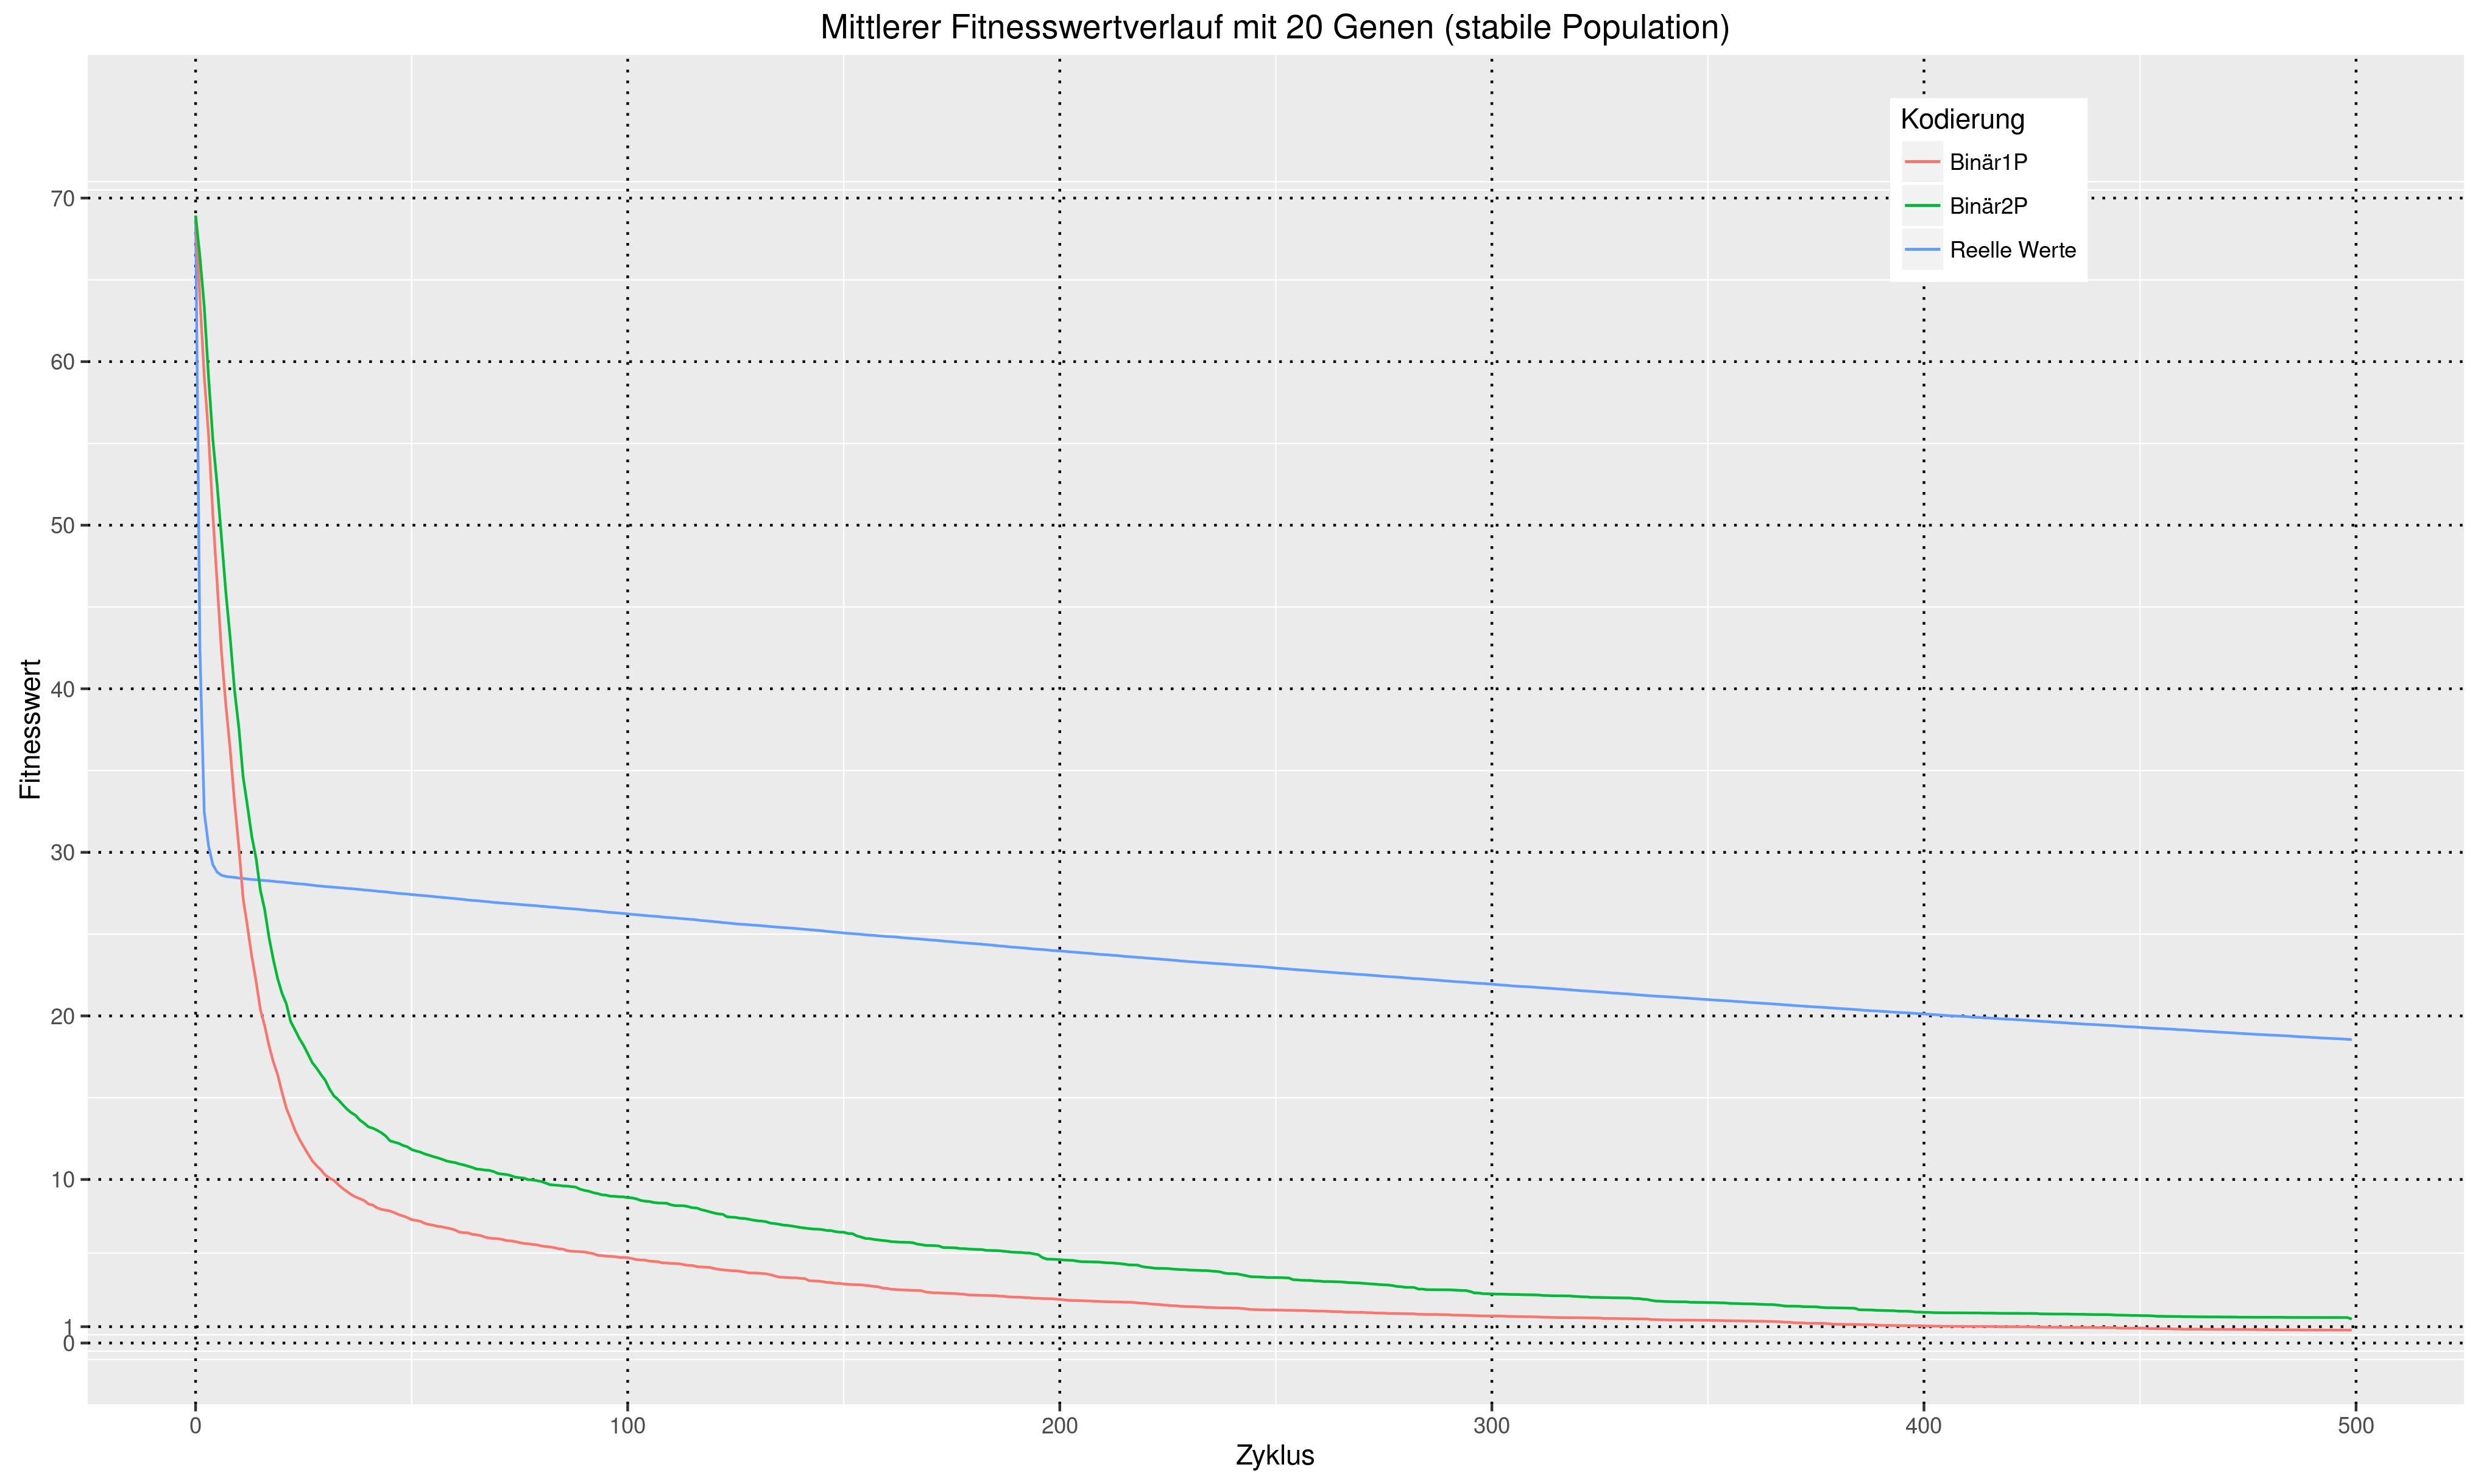
\includegraphics[width=0.75\textwidth]{../best-20-stable.jpeg}
			\caption*{Kodierung im Vergleich bei n=20 (stabile Population)} 
			\label{InputOutput}
		\end{figure}

Ähnliche Ergebnisse werden auch bei einer wachsenden Population erreicht. Im Unterschied zur stabilen Population liefert der Algorithmus aber bessere Ergebnisse für jede Kodierungsart. D.h. es werden in weniger Zyklen bessere Fitnesswerte erreicht, so dass etwa die binären Kodierungsarten bei n=20  das globale Minimum von 0 mit weniger als 200 Zyklen finden (s. nachfolgende Grafik mit n=20). 
	\begin{figure}[H]
	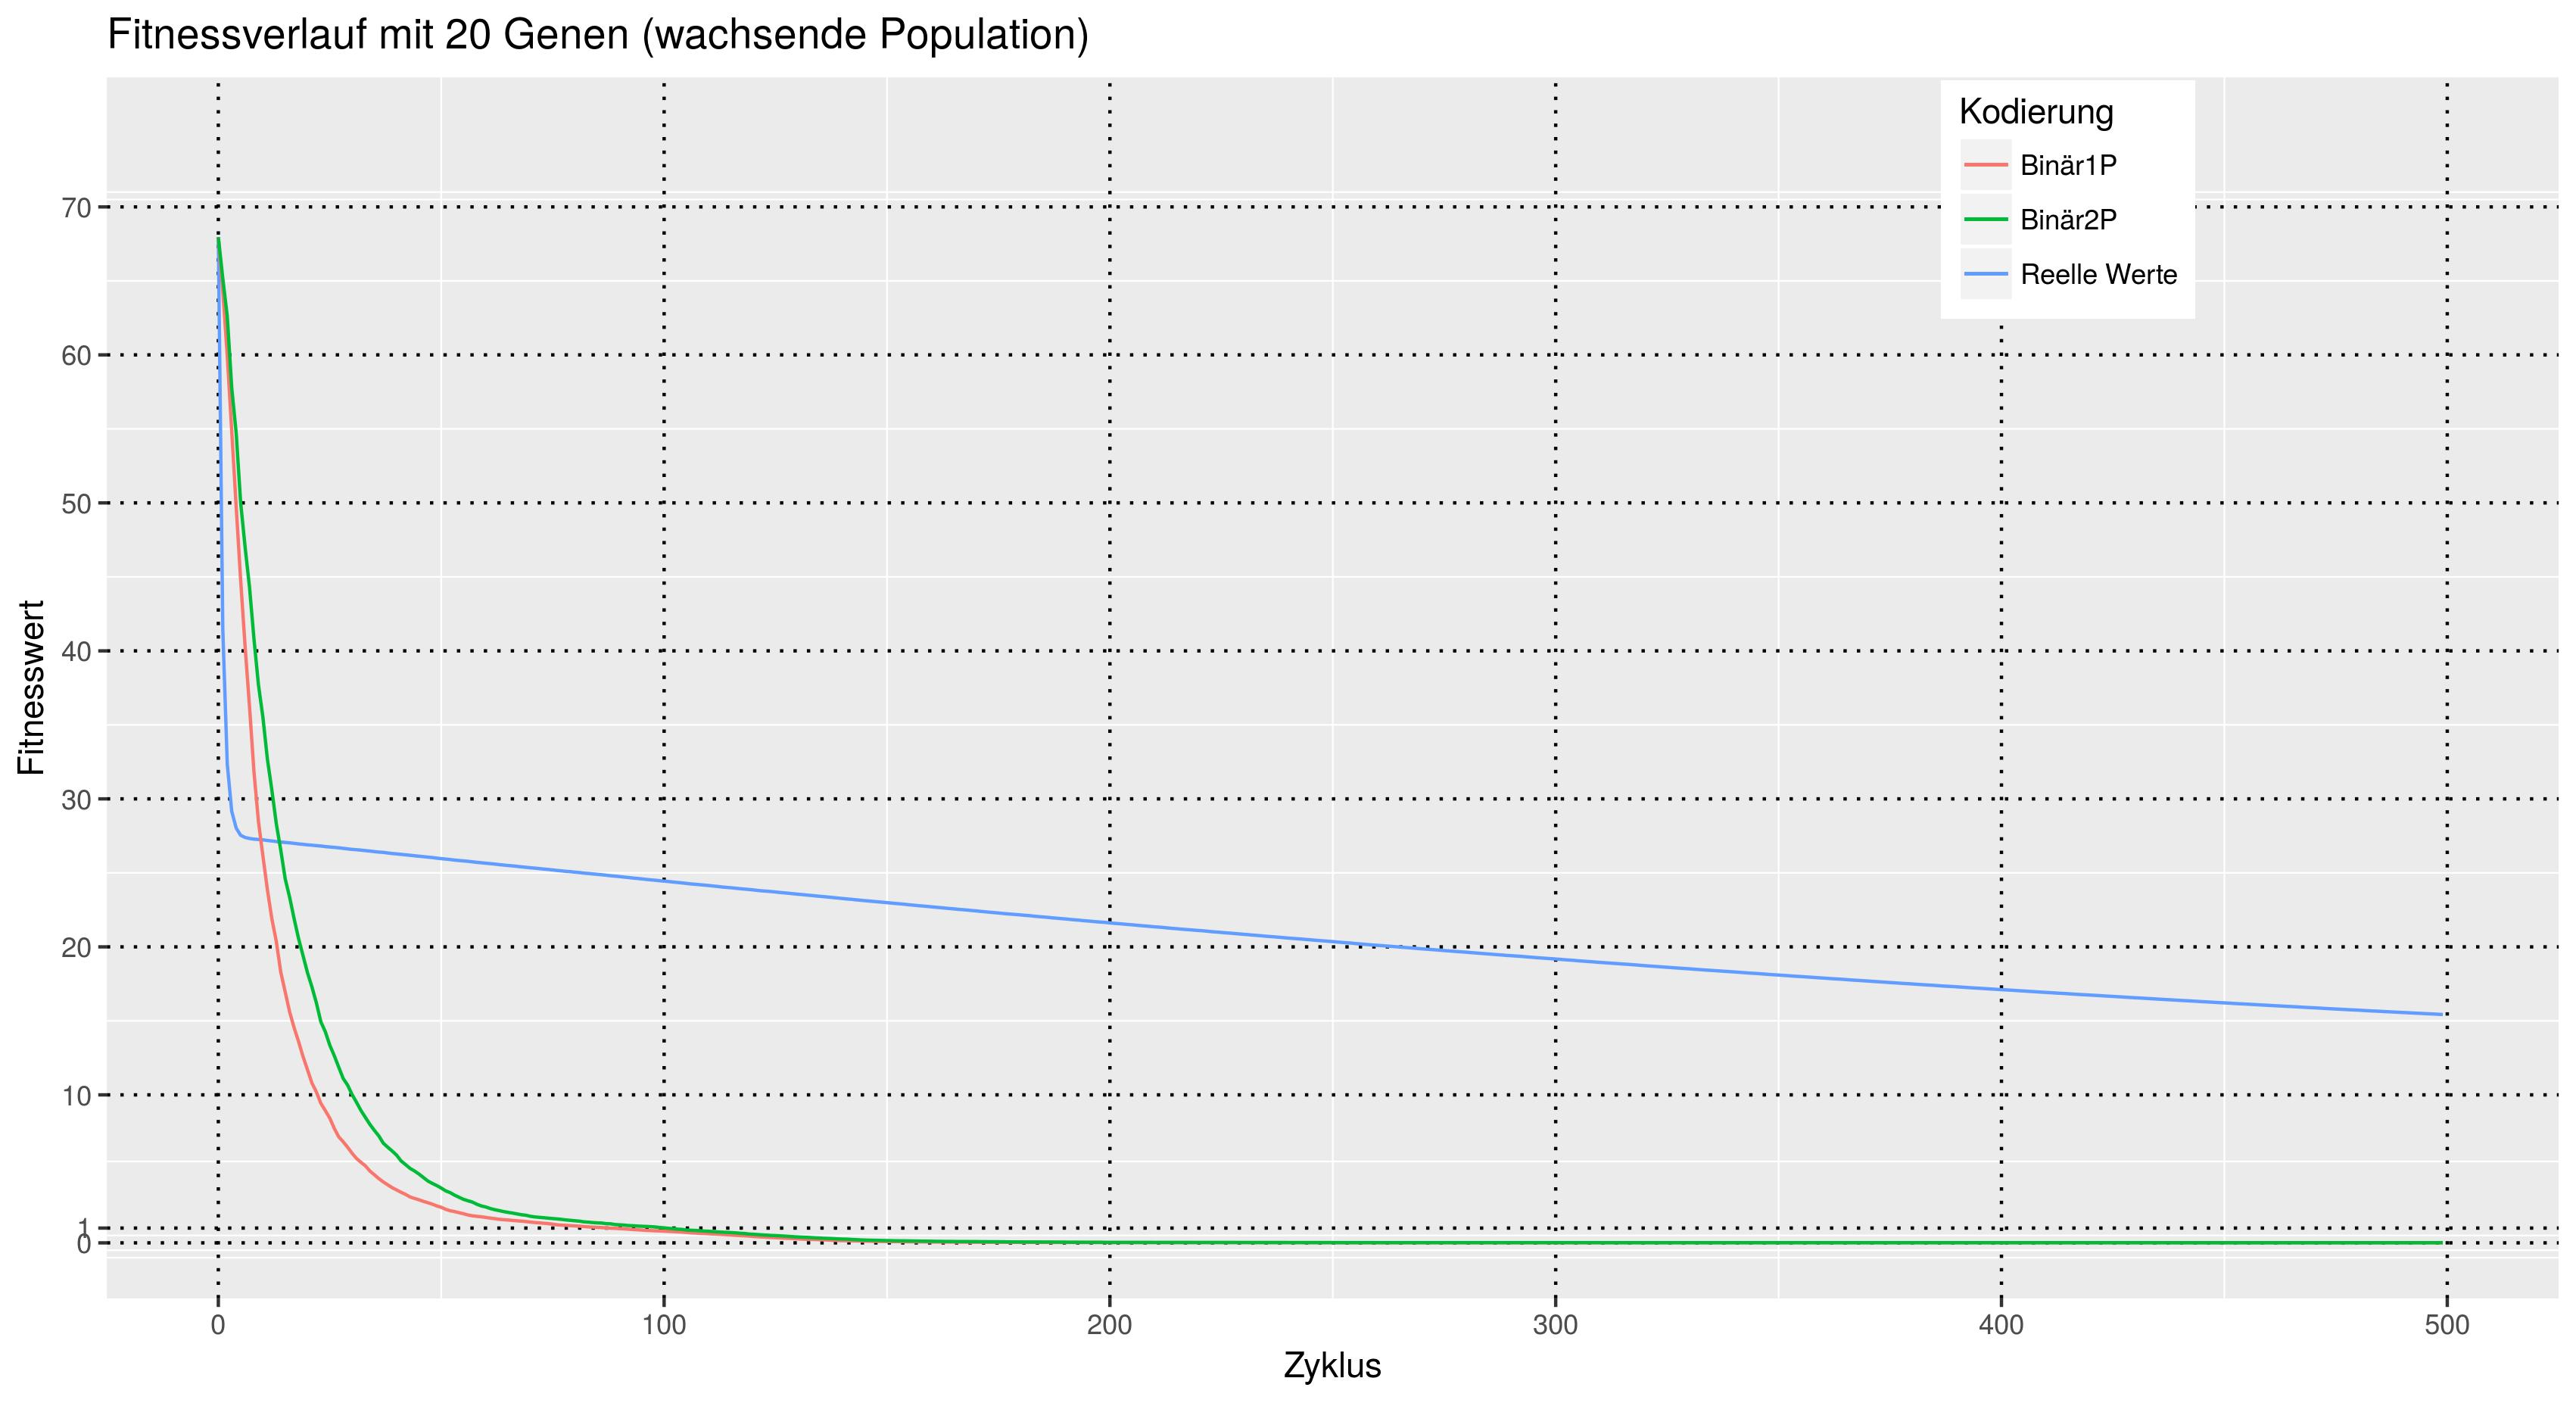
\includegraphics[width=0.75\textwidth]{../best-20-grow.jpeg} 
	
	\caption*{Kodierungen im Vergleich bei n=20 (wachsende Population)} 
	\label{InputOutput}
\end{figure}


Bei Betrachtung der Streuung der Individuen ist auffällig, dass sich bei der reellen Kodierung das schlechteste und das beste Individuum sehr schnell annähern. Bei der binären Kodierung sind die Unterschiede etwas ausgeprägter. Es wird vermutet dass die Streuung maßgeblich für das Ergebnis verantwortlich ist, so dass die besseren Ergebnisse bei den binären Kodierungen aufgrund der größeren Streuung zwischen den Individuen zustande kommen.
		\begin{figure}[H]
		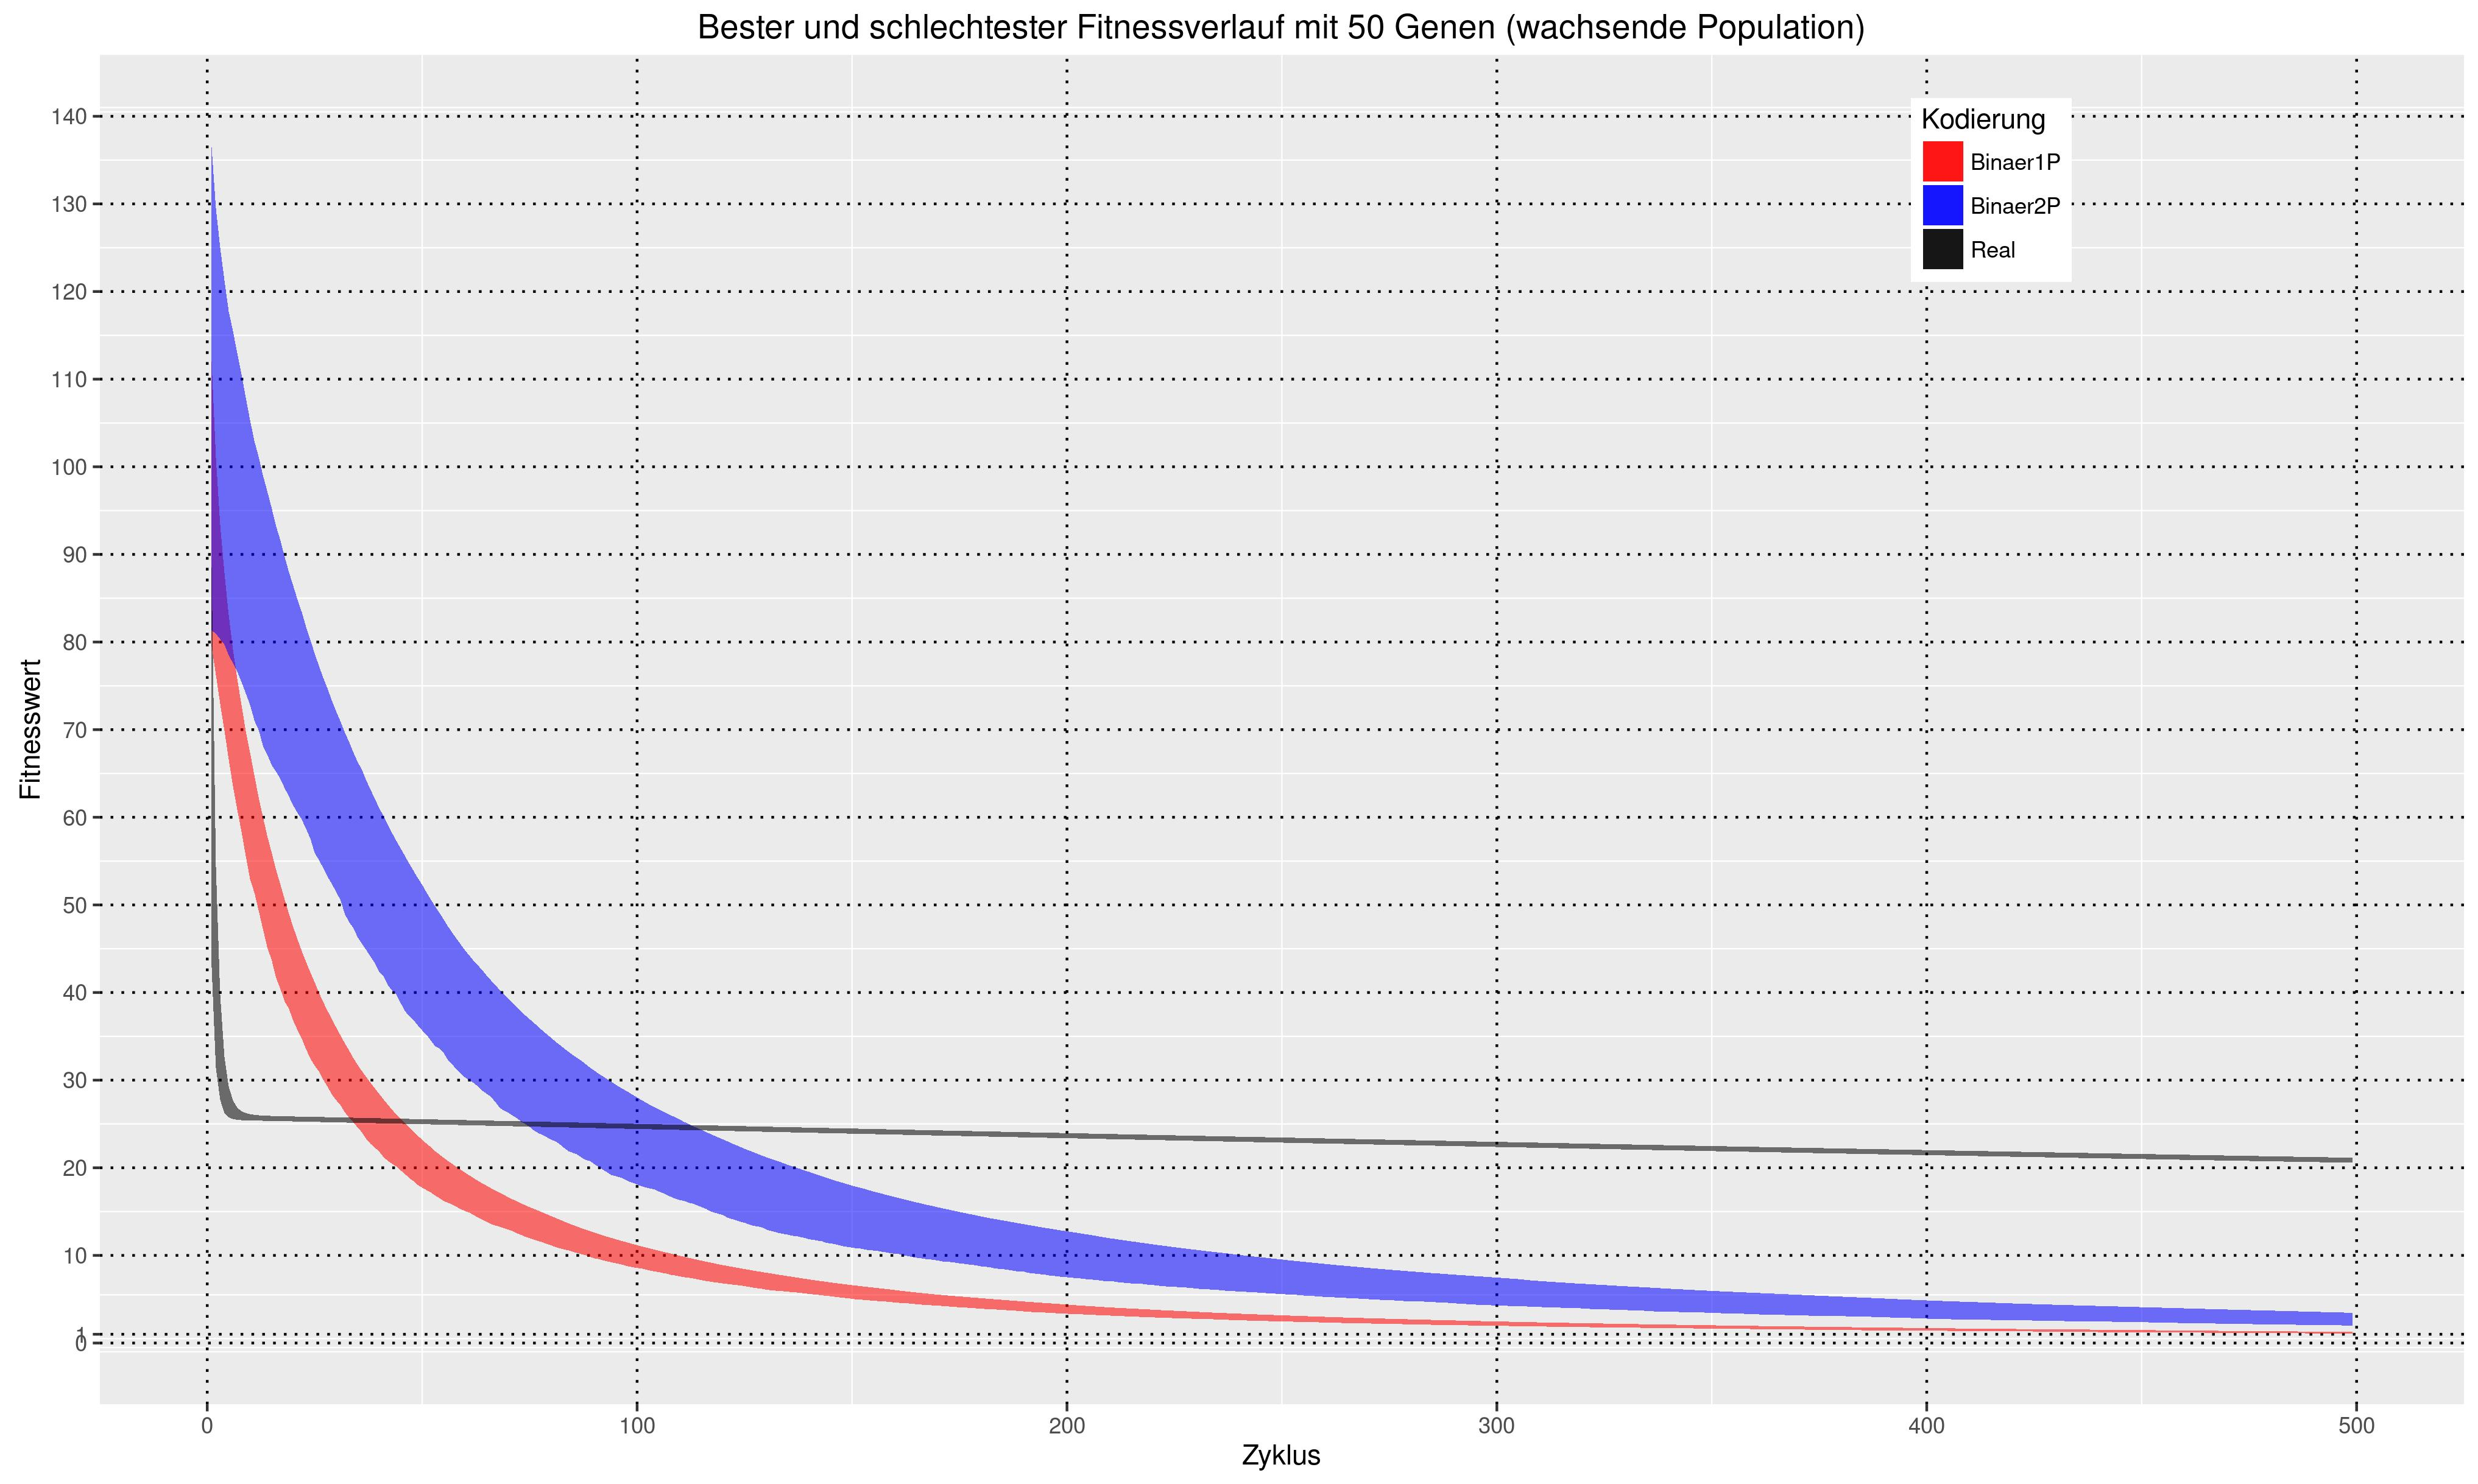
\includegraphics[width=0.75\textwidth]{../best-and-worst.jpeg} 
		
		\caption*{Streuung der Individuen} 
		\label{InputOutput}
	\end{figure}

\begin{figure}[!tbp]
	\centering
	\begin{minipage}[b]{0.45\textwidth}
		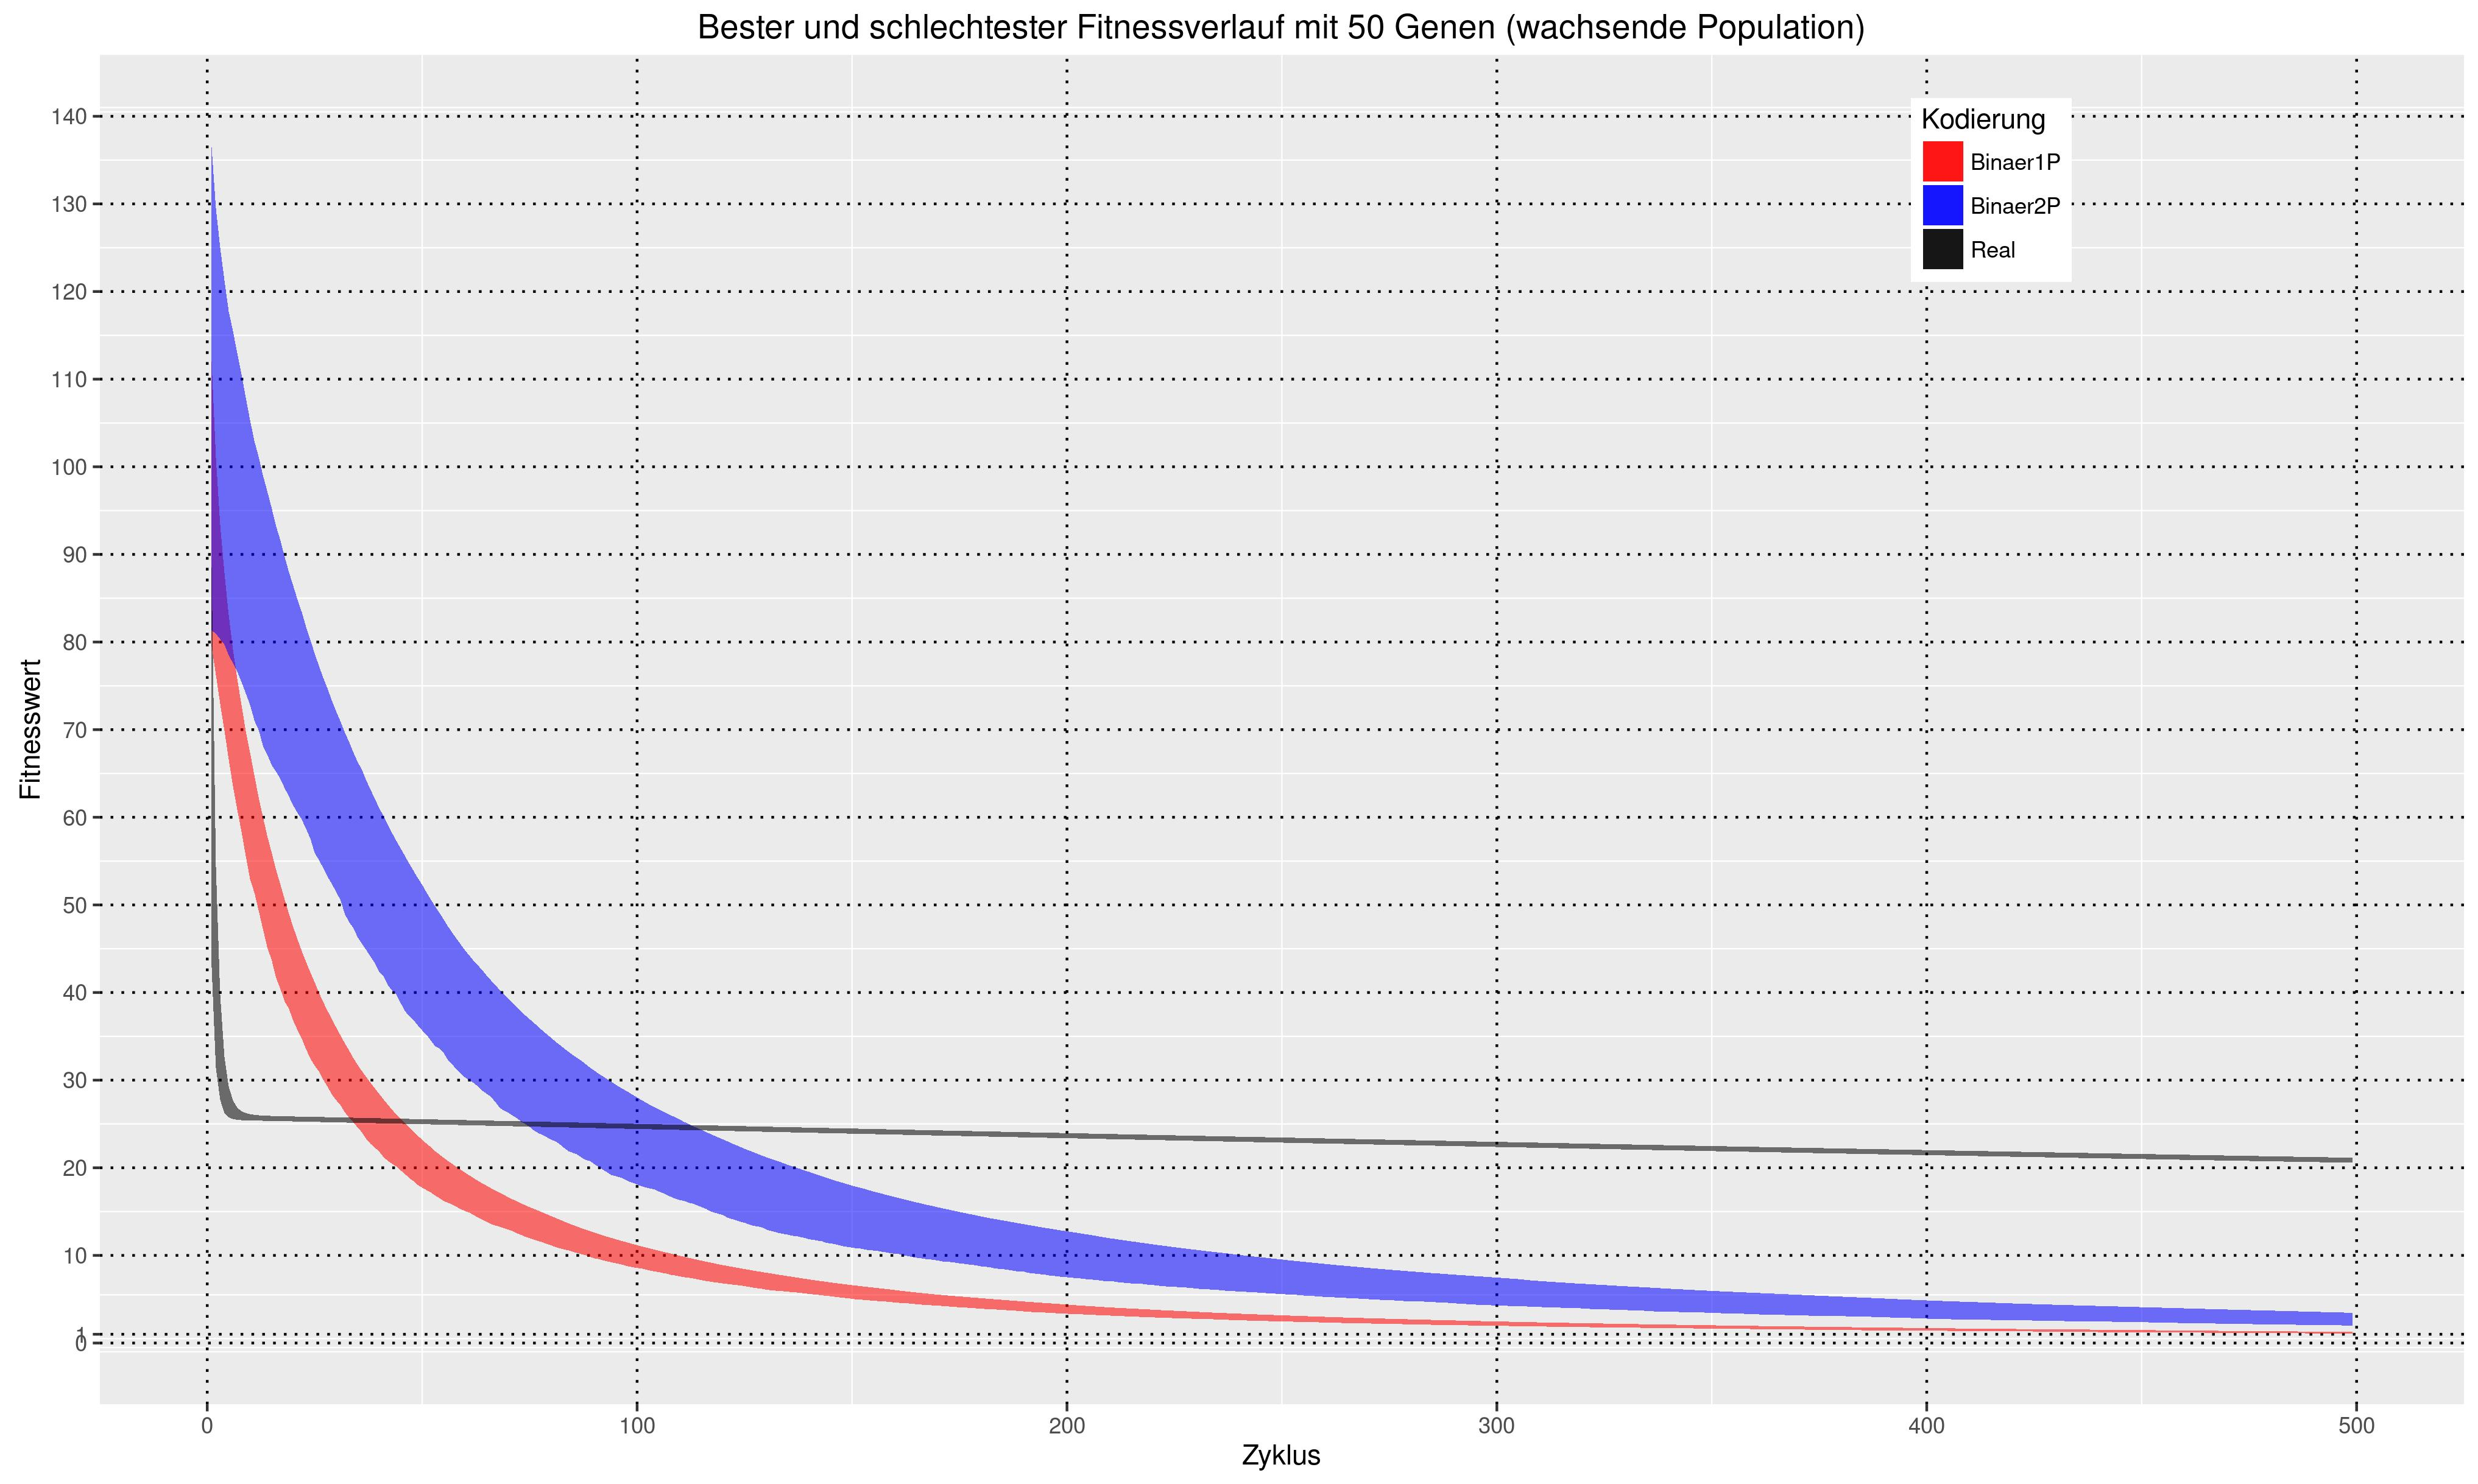
\includegraphics[width=\textwidth]{../best-and-worst.jpeg}
	\end{minipage}
	\hfill
	\begin{minipage}[b]{0.45\textwidth}
		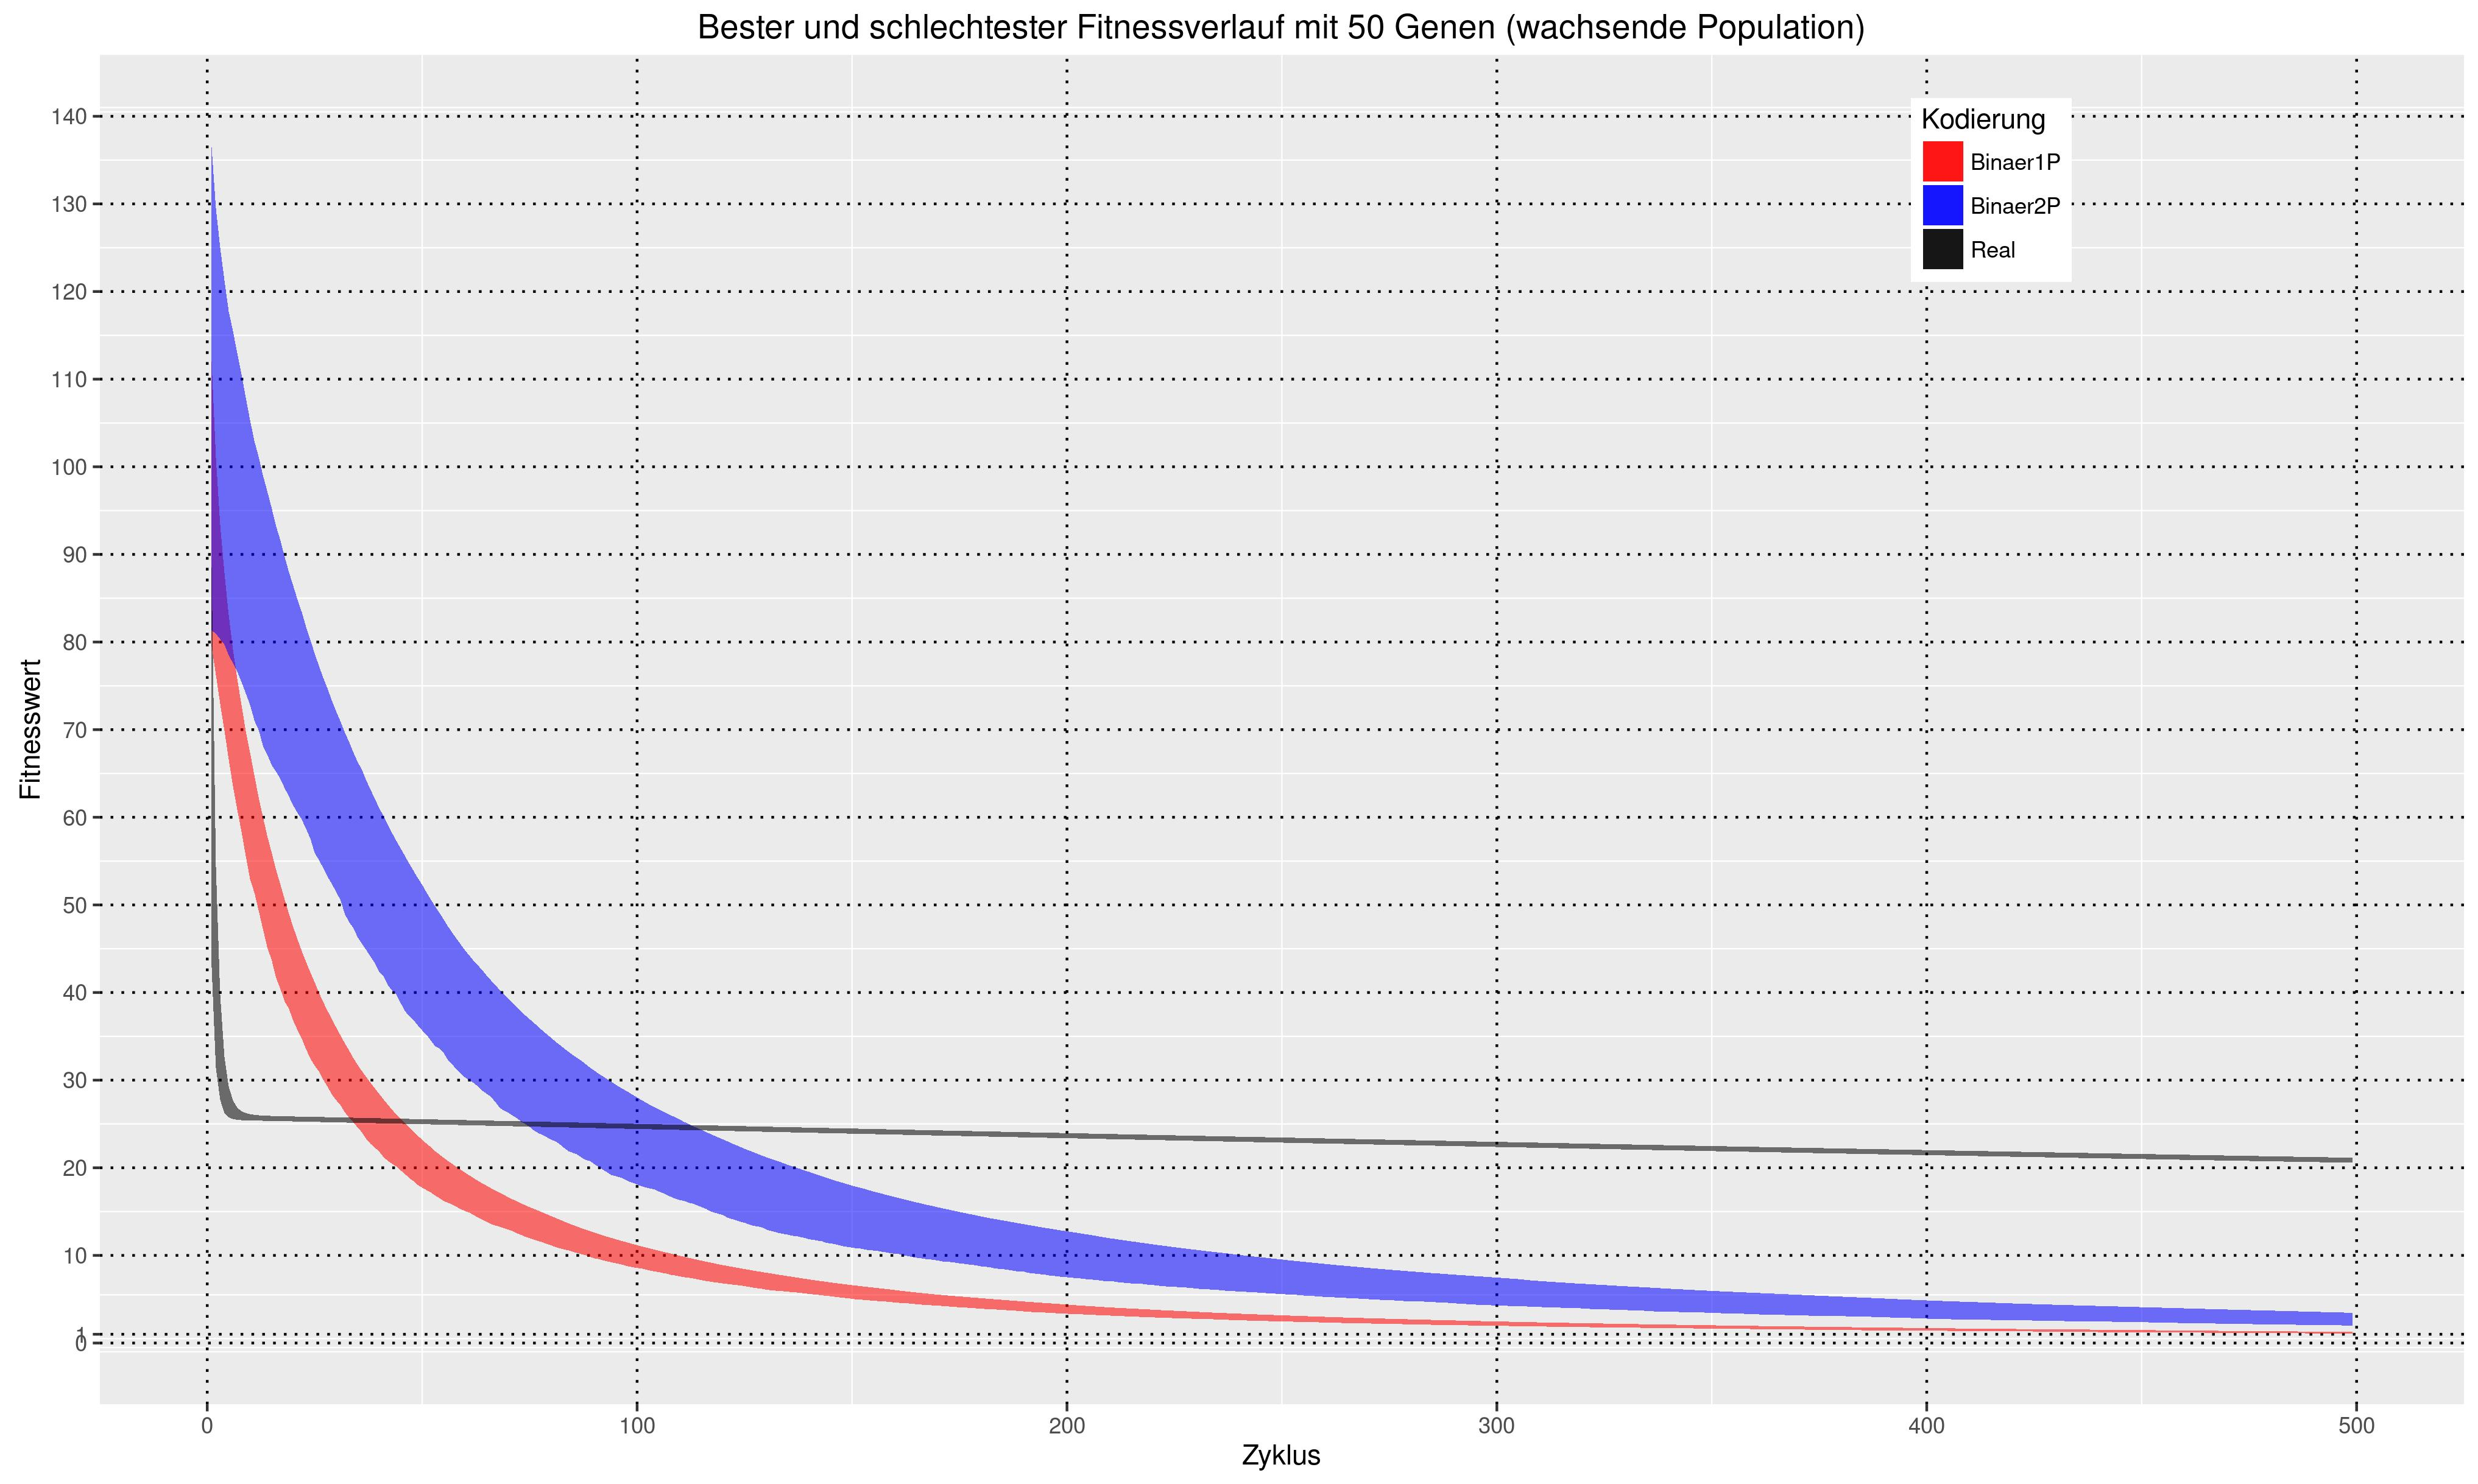
\includegraphics[width=\textwidth]{../best-and-worst.jpeg}
	\end{minipage}
\end{figure}


	
	

	

	
	

	

	


	

	
	
	



%	\glsnogroupskiptrue
%	\printglossary[type=\acronymtype, title=Abkürzungsverzeichnis]
	
%	\listoffigures
%	\addcontentsline{toc}{chapter}{Abbildungsverzeichnis}
	
%	\lstlistoflistings
%	\addcontentsline{toc}{chapter}{Auflistungsverzeichnis}
	
%	\printbibliography 
%	\addcontentsline{toc}{chapter}{Literaturverzeichnis}
	
	
	%\begin{acronym}
	%	\acro{TCP}{Transmission Control Protocol}
	%	\acro{FTP}{File Transfer Protocol}
	%	\acro{IP}{Internet Protocol}
	%	\acro{DNS}{Domain Name Server}
	%	\acro{WWW}{World Wide Web}
%	\end{acronym}

\end{document}